\documentclass[10pt, a4paper]{paper}
\usepackage[ngerman]{babel}
\usepackage{amsmath}
\usepackage{amssymb}
\usepackage{graphicx}
\usepackage{subcaption}
\usepackage{geometry}
\usepackage[utf8]{inputenc}
\usepackage{hyperref}
\usepackage[multiple]{footmisc}
\usepackage{parskip}
\usepackage{wrapfig}
\usepackage{xfrac}
\usepackage{xcolor}
\usepackage{tikz}
\usetikzlibrary{arrows}
\usetikzlibrary{arrows.meta}
\usepackage{longtable}
\usepackage{pdfpages}

\hypersetup{
    colorlinks=true,
    linkcolor=blue,
    filecolor=magenta,      
    urlcolor=cyan
}

\newcommand{\warn}[1]{\textbf{#1}}
\newcommand{\con}[1]{\texttt{#1}}
\newcommand{\dis}[1]{\textbf{\texttt{#1}}}

\title{QRP CW Transceiver Baumappe}
\author{Hannes Matuschek -- DM3MAT\\\texttt{<dm3mat [at] darc [dot] de>}}
\date{\today}

\begin{document}
\maketitle

\begin{abstract}
Dieser multiband Kurzwellen Transceiver deckt alle Bänder von 80m-15m ab und liefert zwischen 2W und 5W. Der Sender besteht aus der PLL (Si5351) die über einen Treiber (74HCT00) die getastete PA (3-4x BS170) ansteuert. Der Empfänger ist ein Direktmischer mit einem sample-hold Mischer (74HCT4052) mit Seitenbandunterdrückung durch die sog. \emph{Phasingmethode}. Die NF Aufbereitung und Verstärkung geschieht durch 12(!) OPVs. Die OPVs sind auch die einzigen Verstärker in der Schaltung. Daher ist auch das Grundrauschen des Empfängers recht hoch. Der Empfänger besitzt auch keinen HF Vorverstärker (ist in Arbeit, wird es als Erweiterung mit AGC geben). Daher sollte gerade auf den oberen Bändern (20m, 17m \& 15m) eine gute Antenne verwendet werden. 
\end{abstract}


\section{Aufbau der Controllerplatine} \label{sec:ctrl}
Zuerst sollte die Controllerplatine aufgebaut und getestet werden. Sie stellt die PLL (Si5351) und Frequenzaufbereitung (74AC74) sowie den Controller (ATMega328) zur Steuerung der PLL und des Displays bereit. 

\begin{table}[!ht]
\centering
\begin{tabular}{|l|l|l|l|}
\hline 
Anz. & Bauteil & Wert & Bemerkung \\ \hline 
5    & R1,R2,R4-R6 & 10k & \warn{R1 Zunächst nicht installieren!} \\
1    & R3 & 1k & \\
1    & RV1 & 10k & Trimmer\\
15   & C1-C3, C5, C9-C19 & 100n & \\
1    & C7 & 10uF & Elko \\
9    & L1-L8 & 100uH & \\
1    & Y1 & 20MHz & Quarz \\
1    & Q1 & 2N3904 & \\
1    & U1 & 74AC74 & ohne Sockel \\
1    & U2 & ATMega328 & mit Sockel! \\
1    & U3 & L7805 & \\
11   & J1-J3, J5-J7, J9, J15-J18 & -- & Stiftleiste 2-Pol \\
1    & J4 & -- & SIP-Sockel für Si5351! \\
1    & J8 & -- & Stiftleiste 3-Pol \\
3    & J10, J13, J14 & -- & Stiftleiste 5-Pol \\
2    & J11, J12 & -- & Stiftleiste 4-Pol \\
1    & (J4) & -- & Si5351 Board \\\hline
\end{tabular}
\caption{Bauteilwerte für die Controllerplatine.}
\end{table}

Beim Aufbau ist zu beachten, \warn{dass der Controller (ATMega328) sowie die PLL (Si5351) mit Sockel installiert werden!} Dies ist nötig damit die Firmware des Controllers später noch verändert werden kann. Die Frequenzaufbereitung (74AC74) kann und sollte jedoch direkt auf die Platine gelötet werden. 

Alle Anschlüsse auf der Controllerplatine (Display, Taste, Drehimpulsgeber, Spannungsversorgung, ...) sollten durch Stiftleisten hergestellt werden. Dies erleichtert den Zusammenbau später.

Der Anschluss J18 (\con{TX-OC}) ist ein optionaler Open-Kollektor Ausgang zur Steuerung einer PA, beim Senden zieht der Transistor Q1 den Ausgang auf Masse.

\warn{Beim Design der Platine und Schaltung ist mir ein Fehler unterlaufen, der verhindert, dass ein Paddle verwendet werden kann. Der Fehler ist in der Firmware behoben, jedoch ist nun die Beschriftung auf der Platine falsch! Der Pin \con{Dit} (J5) auf der Platine ist nun das Resetsignal für das Display (vorher \con{RS} J9) und der Pin \con{Dah} (J10) auf der Platine ist nun das Enablesignal des Displays (vorher \con{EN} J9). Die Pins \con{RS} und \con{EN} (J9) sind nun die funktionierenden Eingänge für das Paddle.}  

\subsection{Test der Frequenzaufbereitung}
Zunächst wird das Display\footnote{Siehe Datenblatt bei Reichelt BNr: \texttt{LCD-PM 2X8-5 A}.} und der Drehimpulsgeber mit der Controllerplatine verbunden. Dazu werden die 4 Datenleitungen zum Display verbunden. \con{D4} auf der Platine zum Pin 11 auf dem LCD, \con{D5} zu Pin 12, \con{D6} zu Pin 13 und \con{D7} zu Pin 14. \warn{\con{Dit} (J5)} auf der Platine wird dann mit Pin 4 und \warn{\con{Dah} (J10)} mit Pin 6 auf dem LCD verbunden. Schließlich folgt noch Anschluss \con{5, C \& G} (5V, Contrast, GND auf Stiftleiste J8) mit den Pins 2, 3 \& 1 auf dem LCD. Das Display ist nun angeschlossen. Der Kontrast des LCD lässt sich dann über den Widerstand RV1 einstellen. \warn{Pin 5 und 2 des LCDs müssen noch direkt miteinander verbunden werden.}

Der Drehimpulsgeber\footnote{Siehe Datenblatt bei Reichelt BNr: \texttt{STEC11B13}.} wird mit \con{RotA, RotB \& RotC} und Masse verbunden (ein Pin der Stiftleiste J12) verbunden, wobei \con{RotA} \& \con{RotB} mit den entsprechenden Pins des Drehimpulsgebers (meist \con{A} und \con{B} genannt) und \con{RotC} mit dem Pin des Achsentasters verbunden wird. 

Zuletzt wird die Spannungsversorgung (13.8V) an \con{J3} oder \con{J17} hergestellt. \warn{Diese Platine besitzt keine Verpolschutzdiode! Daher unbedingt auf den polrichtigen Anschluss achten!}

Wenn alles stimmt, sollten Sie nun im Display die Frequenzanzeige \dis{3500.00} sehen und in der unteren Zeile des Displays \dis{AR}. Nun können Sie sich mit der Menüführung (siehe Abschnitt \ref{sec:user}) vertraut machen. 

Zum Test der Frequenzaufbereitung benutzen Sie ein Oszilloskop mit Frequenzzähler. Am Anschluss \con{I} (J2) und \con{Q} (J1) sollten Sie eine um 700Hz geringere Frequenz als im Display angezeigt wird ablesen können. Falls Ihr Oszilloskop über zwei Kanäle verfügt, können sie auch die Phasenverschiebung zwischen den beiden Signalen \con{I} und \con{Q} überprüfen. 

Wenn Sie nun den Anschluss \con{RS} (J9) mit einer Krokodilklemme mit Masse verbinden, sollte am Anschluss \con{TxOsc} (J16) die eingestellte Frequenz messbar und die Ausgänge \con{I} und \con{Q} abgeschaltet sein. Damit ist der Test der Frequenzaufbereitung und der Controllerplatine abgeschlossen. Es folgt der Aufbau der PA.

\subsection{S-Meter oder Betriebsspannung?} \label{sec:meter}
Aus Ermangelung freier Pins am Controller kann nur ein Pin für Messungen verwendet werden. Entweder als S-Meter oder zur Messung der Betriebsspannung z.B. für den Portabelbetrieb mit Akku. 

In der Schaltung vorgesehen ist das S-Meter. Dazu wird R1 auf der Controllerplatine installiert und der Pin \con{SMe} (J5) später mit dem Pin \con{S} (J4) auf der Empfängerplatine verbunden. Dieses S-Meter ist sehr ungenau und die Beurteilung der Signalstärke ist durch die fehlende AGC auch mit dem Ohr machbar.

Wenn der TRX im Portabelbetrieb verwendet werden soll, ist eine Messung der Betriebsspannung deutlich hilfreicher, um den Ladestand der Batterie beurteilen zu können. Der S-Meter Pin (\con{SMe}, J5) lässt sich daher auch zur Messung der Betriebsspannung verwenden. 
Dazu wird R1 \warn{nicht} eingebaut. Und es müssen zwei Widerstände \emph{fliegend} Installiert werden. Ein 1k Widerstand wird dazu zwischen den \con{SMe} Pin und Masse (z.B. an J12 direkt dahinter eingelötet. Dann wird ein 10k Widerstand mit Schrumpfschlauch-Isolierung von Pin \con{SMe} zur Spannungsversorgung, z.B. an J3, J17 oder auch an ein Bein von L2 geführt. 

Die von Ihnen gewählte Konfiguration muss dann noch im Setup Menu unter \emph{Meter} eingestellt werden.


\clearpage
\section{Aufbau der PA-Platine} \label{sec:pa}
\begin{table}[!ht]
 \begin{tabular}{|p{1cm}|p{6cm}|p{2cm}|p{3cm}|} \hline 
 Anz. & Bauteil & Wert & Bemerkung \\ \hline
 7  & R1, R3, R5, R7, R11, R15, R16 & 10k & \\
 4  & R2, R4, R6, R8 & 100k & \\
 1  & R9 & 470 & \\
 1  & R10 & 1k & \\
 2  & R12, R13 & 100 & \\
 1  & R14 & 4.7k & \\
 
 9  & C1, C10, C19, C20, C22-C24, C26, C27 & 100n & \\
 2  & C2, C15 & 100p & NP0 \\
 2  & C3, C16 & 150p & NP0 \\
 4  & C4, C17, C7, C12 & 330p & NP0 \\
 2  & C5, C18 & 470p & NP0 \\
 2  & C8, C13 & 680p & NP0 \\
 2  & C6, C11 & 220p & NP0 \\
 2  & C9, C14 & 1.0n & NP0 \\
 1  & C21 & 1.0n & Keramik\\ 
 1  & C25 & 1u & Keramik \\
 1  & C28 & 100u & Elko \\
 
 2  & L1, L9 & 440nH & 12T T37-6\\
 2  & L2, L10 & 650nH & 15T T37-6\\
 2  & L3, L11 & 1330nH & 18T T37-2\\
 2  & L4, L12 & 2050nH & 23T T37-2\\
 1  & L5 & 520nH & 13T T37-6\\
 1  & L6 & 760nH & 16T T37-6\\
 1  & L7 & 1530nH & 20T T37-2\\
 1  & L8 & 2400nH & 25T T37-2\\

 1  & T1 & --- & Siehe Text.\\ 
 
 4  & D1-D3,D5 & 1n4148 & \\
 1  & D4 & 1N4001 & \\

 4  & Q1-Q3, Q10 & 2N3904 & \\
 6  & Q4, Q6-Q9 ,Q11 & BS170 & \\
 1  & Q5 & BD140 & \\

 1  & U1 & 74HCT00 & \\
 1  & U2 & L78L05 & \\

 4  & K1-K4 & FINDER-30.22 & \\

 1  & J1 & BNC & \\

 11 & J2-J12 & --- & Stiftleiste 2-Pol \\ \hline
 \end{tabular}
 \caption{Bauteilwerte der PA Platine.} \label{tab:pa}
\end{table}

Die PA und Tiefpassfilter Platine beheimatet nicht nur die PA und Tiefpassfilterschaltung sondern auch den Treiber (75HCT00), Sende/Empfangsumschalter (Q4) und die PA-Tastung und Keyshaping (Q5 \& Q8).

Der Aufbau ist soweit recht unkritisch, \warn{jedoch müssen die Spulen für den Tiefpass gewickelt und ausgemessen werden!} Außerdem ist es Hilfreich die BNC-Buchse zunächst nur mit den zwei Anschlusspins zu verlöten. \warn{Die Befestigungspfosten der Buchse sollten noch nicht verlötet werden!} Dies geschieht erst, wenn die PA Platine in das Gehäuse eingebaut wird. 

Die Kondensatoren der Tiefpässe befinden sich zusammen mit den Ringkernen in einer extra Tüte. Diese Kondensatoren sind vom Typ NP0 und besitzen eine höhere Genauigkeit und Temperaturstabilität gegenüber anderen Vielschicht- oder Scheibenkondensatoren. Sind aber deutlich günstiger als Glimmerkondensatoren (Faktor 10 oder so).

Damit die Spulen der Tiefpässe die korrekten Werte besitzen, werden zunächst 1-2 Windungen mehr auf die Kerne gebracht als in Tabelle \ref{tab:pa} angegeben und dann die resultierenden Spulen mit einer LCR Brücke vermessen. Gegebenenfalls werden dann Windungen abgenommen bis die gewünschte Induktivität in etwa erreicht wird. Zum Schluss kann die Induktivität dann noch leicht durch zusammendrücken oder auseinanderziehen der Windungen verändert werden. 

Für den 15m \& 17m Tiefpass sind L1 \& L9 je 440nH mit c.a. 12 Windungen (2 x 23 cm 0.5mm CuL\footnote{Die Drahtlängen berücksichtigen schon c.a. 2.5cm \emph{pig-tails} (Drahtenden) sowie zwei extra Windungen, die gegebenenfalls wieder entfernt werden müssen, um die gewünschte Induktivität zu erreichen.}) und L5 520nH mit c.a. 13 Windungen (24 cm 0.5mm CuL) auf einem T37-6 Kern (gelb). 

Für den 20m \& 30m Tiefpass sind L2 \& L10 je 650nH mit c.a. 15 Windungen (2 x 28 cm 0.5mm CuL) und L6 760nH mit c.a. 16 Windungen (29 cm 0.5mm CuL) auf einem T37-6 Kern (gelb).

Für den 40m \& 60m Tiefpass sind L3 \& L11 je 1330nH mit c.a. 18 Windungen (2 x 31 cm 0.3mm CuL) und L7 1530nH mit c.a. 20 Windungen (33 cm 0.3mm CuL) auf einem T37-2 Kern (rot).

Für den 80m Tiefpass sind L4 \& L12 je 2050nH mit c.a. 23 Windungen (2 x 37 cm 0.3mm CuL) und L8 2400nH mit c.a. 25 Windungen (39 cm 0.3mm CuL) auf einem T37-2 Kern (rot).

Damit die Ringspulen alle gut auf die Platine passen und sich nicht gegenseitig berühren, \warn{muss auf den Wickelsinn geachtet werden!} Alle Spulen L1-L8 werden wie folgt gewickelt: Die Windungen werden \textbf{gegen den Uhrzeigersinn} aufgebracht wobei das erste Ende des Drahtes zunächst \textbf{von Vorn durch den Kern gesteckt wird} und dann die Windungen aufgetragen werden. 

\warn{Der Transformator T1 wird genau andersherum gewickelt!} Es werden die Windungen zwar auch gegen den Uhrzeigersinn aufgetragen, jedoch wird das erste Ende des Drahtes \textbf{von Hinten durch den Kern gesteckt} und dann die Windungen aufgetragen. 

\begin{wrapfigure}{l}{3cm}
 \centering
 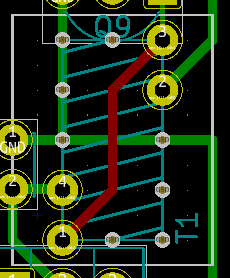
\includegraphics[width=2.5cm]{fig/T1.png}
 \caption{T1 auf der PA Platine.} \label{fig:T1}
\end{wrapfigure}
Der Transformator T1 bestimmt auch die Ausgangsleistung des Transceivers. Er ist als Autotransformator verschaltet. Die Primärseite hat immer 8 Windungen (15 cm 0.5mm CuL) auf einem FT37-43 (schwarz) Kern. Werden \textbf{keine} Sekundärwindungen aufgetragen wird die Ausgangsleistung c.a. 1.5-2W betragen bei 12-13.8V Betriebsspannung. Werden dann 8 Sekundärwindungen aufgetragen, kann die Ausgangsleistung c.a. 6-7W betragen bei 12-13.8V Betriebsspannung (in der Realität eher 4-6W). 

Die Anschlüsse des Transformators auf der Platine sind nummeriert und in Abbildung \ref{fig:T1} dargestellt: \con{1} (links Unten), \con{4} (links Mitte), \con{2} (rechts Mitte), \con{3} (rechts Oben). Die Primärspule geht von \con{4} nach \con{3} und die Sekundärspule von \con{1} nach \con{2}. 

Zum Testen der PA sollte zunächst keine Sekundärwicklung aufgebracht werden. D.h., T1 ist dann nur eine Spule mit 8 Windungen auf dem FT37-43 Kern, wobei ein Ende durch Loch \con{4} und das andere Ende durch Loch \con{2} auf der Platine gesteckt und verlötet wird. Danach werden die Löcher \con{2} und \con{3} (rechts Mitte und Oben) mit einer Brücke aus Lötzinn miteinander Verbunden. Später kann dann der Transformator T1 mit dem gewünschten Windungsverhältnis (siehe Tabelle \ref{tab:Pout}) installiert werden.

\begin{table}[!ht]
 \centering
 \begin{tabular}{|l|l|l|l|l|} \hline
  Primär & Sekundär & Pwr (9V) & Pwr (12V) & Pwr (13.8V) \\ \hline
  8 & 0 & 0.8 & 1.4 & 1.9 \\
  8 & 1 & 1.0 & 1.8 & 2.4 \\
  8 & 2 & 1.3 & 2.2 & 3.0 \\
  8 & 3 & 1.5 & 2.7 & 3.6 \\
  8 & 4 & 1.8 & 3.2 & 4.3 \\
  8 & 5 & 2.1 & 3.8 & 5.0 \\
  8 & 6 & 2.5 & 4.4 & \warn{5.8} \\
  8 & 7 & 2.8 & \warn{5.1} & \warn{6.7} \\
  8 & 8 & 3.2 & \warn{5.8} & \warn{7.6} \\ \hline 
 \end{tabular}
 \caption{Theoretische maximale Ausgangsleistungen für bestimmte Windungsverhältnisse auf T1 und verschiedenen Betriebsspannungen. \warn{Werden mehr als 5W Ausgangsleistung erwartet, sollte auch der vierte PA Transistor Q11 Installiert werden. Für Ausgangsleistungen kleiner 5W genügen drei (Q6,Q7,Q9) MosFETs.}} \label{tab:Pout} 
\end{table}


\subsection{Test der PA-Platine}
Zum Testen der PA Platine werden \con{TX 5V} (J10) und \con{Key} (J5) der PA Platine mit \con{T} und \con{K} (J6) auf der Controllerplatine verbunden. Dann wird die Spannungsversorgung der PA Platine (J8 oder J12) von J3 oder J17 der Controllerplatine durchgeschleift. Danach werden die Tiefpassfiltersteuersignale \con{10}, \con{20}, \con{40} und \con{80} (J13) von der Controllerplatine zu den jeweiligen Bandpassfiltern (J9, J2, J3, J4) auf der PA-Platine geführt.

Mit einem kurzen Stück RG-174 wird dann das \con{TxOsc} Signal von der Controllerplatine zur Vorstufe \con{TX HF} auf der PA Platine geführt.

Zuletzt wird die Stromversorgung der Endstufe (J11) direkt mit der Spannungsversorgung Verbunden.  \warn{Achten Sie bei der Spannungsversorgung auf den polrichtigen Anschluss!} Die Verpolschutzdiode D4 ist durch einen Designfehler wirkungslos! Sie sollte nicht parallel zu J8 und J12 sonder parallel zu J11 sein. Wenn Sie nicht auf eine Verpolschutzdiode verzichten wollen, befestigen Sie D4 in Sperrrichtung direkt an der Hohlsteckerbuchse.

\warn{Bevor die Schaltung in Betrieb genommen wird, muss ein Dummyload an die BNC Buchse angeschlossen werden!}

Wenn Sie nun wieder \con{RS} (J9, Controllerplatine) mit Masse verbinden, sollte der TRX senden und c.a. 1.9W in das Dummyload abgeben.  Prüfen sie auch die Signalform am Dummyload und das Keyshaping der Tastung.

Verhält sich die Schaltung vernünftig, können sie T1 mit dem gewünschten Windungsverhältnis bewickeln (siehe Tabelle \ref{tab:Pout}) und in die PA einbauen. Prüfen Sie nach dem Austausch von T1 nochmal die Signalform am Dummyload. 

Ist der Endstufentest abgeschlossen, kann nun mit dem Aufbau des Empfängers begonnen werden. 
 
\subsubsection{(Optional) Abgleich der Tiefpassfilter}
Um die Tiefpassfilter final fein abzustimmen, wird ein Spektrumanalyzer mit Trackinggenerator, Wobbler oder Netzwerkanalyzer benötigt. 

Zunächst wird zur Sicherheit die Spannungsversorgung der Endstufentransistoren (J11) getrennt. Danach wird eine 100uH Festinduktivität über dem \con{RX HF} (J6) Anschluss gelötet. Diese Induktivität simuliert den benötigten Eingangstransformator des Empfängers, damit die Sen\-de/Emp\-fangs\-um\-schal\-tung (Q4) funktioniert. Das Ausgangssignal des Analyzers/Wobblers wird dann mit der BNC Buche verbunden. Das gefilterte Signal kann dann über der temporären Induktivität an \con{RX HF} (J6) abgegriffen werden. Die Tiefpassfilter können nun durch auseinanderziehen oder zusammendrücken der Windungen der Filterspulen leicht abgeglichen werden. 


\clearpage
\section{Aufbau der Empfängerplatine} \label{sec:rx}
Der Aufbau der Empfängerplatine ist unkritisch, da der einzige Bereich der Platine mit HF die linke obere Ecke um den 74HC4052 ist. Der Rest der Platine ist nur NF Aufbereitung, Filter und Verstärkung. Daher können die OPVs auch auf IC-Sockel montiert werden um später bessere oder defekte OPVs austauschen zu können. 

\begin{table}[!ht]
 \begin{tabular}{|p{1cm}|p{6cm}|p{2cm}|p{3cm}|} \hline 
 Anz. & Bauteil & Wert & Bemerkung \\ \hline
 2  & R1, R4 & 30k & \\
 8  & R3, R6, R7, R18, R19, R23, R26, R28 & 10k & \\
 2  & R8, R10 & 33k & \\
 1  & R11 & 120k & \\
 2  & R12, R17 & 36k & \\
 4  & R13-R16 & 100 & \\
 2  & R20, R22 & 4.7k & \\
 3  & R21, R40, R41 & 1k & \\
 1  & R24 & 5.1k & \\
 9  & R9, R25, R27, R29, R30, R33, R35, R38, R39 & 3.3k & \\
 1  & R31 & 470k & \\
 1  & R32 & 4.3k & \\
 1  & R34 & 7.5k & \\
 2  & RV1, RV2 & 50k & Timmer\\
 1  & RV3 & 500 & Timmer \\

 14 & C1-C3, C5, C6, C8-C10, C14, C19, C20, C23, C29, C37 & 100n & \\
 4  & C4, C11, C21, C33 & 47n & \\
 3  & C7, C16, C28 & 1n & \\
 6  & C12, C22, C24, C27, C35, C38 & 10u & Elko \\
 5  & C13, C15, C17, C18, C36 & 470n & \\
 4  & C25, C26, C30, C34 & 10n & \\
 3  & C31, C32 & 3.3n & \\

 1  & L1 & 470u & \\
 1  & T1 & 3 x 12.6uH & 6 Wind. trifilar auf FT37-43 \\

 1  & D1 & 1N4148 & \\ 
 1  & Q1 & BS170 & \\

 5  & U1-U3, U6, U7 & LM833 & In Sockel! \\
 1  & U4 & 74HC4052 & \\
 1  & U5 & TLC272 & In Sockel! \\
 1  & U8 & L78L05 & \\

 7  & J1, J2, J5-J9 & --- & Stiftleiste 2-Pol\\ 
 1  & J3 & --- & Stiftleiste 3-Pol \\
 1  & J4 & --- & Stiftleiste 4-Pol \\\hline
 \end{tabular}
 \caption{Bauteilwerte der Empfängerplatine.}
\end{table}

Beim Wickeln des Eingangstransformators T1 \warn{muss wieder auf den Windungssinn geachtet werden!} Es werden 6 Windungen trifilar (3 x 13 cm 0.5 mm CuL) auf den Kern gebracht, indem drei Stücke CuL-Draht verdrillt und dann \textbf{gegen den Uhrzeigersinn} auf den Kern gewickelt werden. Sie beginnen die erste Windung, indem Sie das Ende des Drahtes \textbf{von Hinten durch den Kern stecken}.

\subsection{Abgleich}
Verbinden Sie zunächst den HF Eingang \con{RF} (J2) auf der Emp\-fän\-ger\-pla\-ti\-ne mit \con{RX HF} (J6) auf der PA-Platine mit einem Stück RG-174. Danach werden \con{I} \& \con{Q} (J6 \& J7) auf der Empfängerplatine mit den Ausgängen \con{I} \& \con{Q} (J2 \& J1) auf der Controllerplatine mit zwei Stücken RG-174 verbunden. 

Verbinden Sie dann die Kopf\-hö\-rer\-buch\-se mit \con{HP} (J5) mit dem Audiokoaxialkabel und das Lautstärke Poti mit \con{Vol} (J3) mit dem zweiadrigen geschirmten Audiokabel. Verbinden Sie dann \con{TX5V} (J8) auf der Empfängerplatine mit \con{T} (J15) auf der Controllerplatine. Verbinden Sie dann \con{T} (J4) auf der Empfängerplatine mit \con{ST} (J13) auf der Controllerplatine mit einem Stück Audiokoaxialkabel. 

Schleifen sie dann die Spannungsversorgung des Empfängers von der PA-Platine (J8 oder J12) zur Empfängerplatine (J1 oder J9) durch. \warn{Achten Sie auf den polrichtigen Anschluss!}

Wenn alles gut gegangen ist, sollten Sie nun bei voll aufgedrehter Lautstärke Rauschen im Kopfhörer hören. 

Im Folgenden werde ich den Abgleich der Audiophasenverschiebung zur Seitebandunterdrückung beschreiben. Meiner Erfahrung nach ist die Seitenbandunterdrückung bei weitem nicht perfekt. Auch wenn Sie eine nahezu ideale Seitenbandunterdrückung auf einem Band bekommen, wird sie auf einem anderen Band deutlich schlechter sein. Es ist also nötig beim Abgleich immer wieder die Bänder zu wechseln und ein gutes Mittelmaß für die für Sie interessanten Bänder zu finden. 

Schließen Sie zunächst einen Signalgenerator mit geringer Ausgangsleistung oder mit Hilfe eines geeigneten Dämpfungsgliedes an den Eingang des TRX. Stellen sie am Signalgenerator eine Frequenz innerhalb eines Amateurfunkbandes ein (z.B., 14010.00kHz). Stimmen sie nun den Empfänger auf eben jene Frequenz ab. Erhöhen oder verringern sie die Leistung des Signalgenerators oder wählen sie die Dämpfung des Dämpfungsgliedes so, dass ein lauter Ton im Kopfhörer zu hören ist. Stimmen sie nun den Empfänger auf eine 1.4kHz höhere Frequenz ab (für das vorherige Beispiel wäre es dann 14011.4kHz). Wenn sie nun einen (leiseren) Ton hören, versuchen sie mit Hilfe der Einstellwiderständen RV1, RV2 und RV3 die Lautstärke dieses Tons zu minimieren. Es ist möglich für ein Band diesen Ton vollständig zum Verschwinden zu bringen. Jedoch wird dadurch die Seitenbandunterdrückung auf anderen Bändern schlechter. Sie müssen also immer wieder das Band wechseln und die Prozedur von vorn beginnen, bis sie ein über mehrere Bänder akzeptables Ergebnis erreichen. 

Testen sie den Empfänger und Sender ruhig schon mal auf dem Band. Wenn alles zu Ihrer Zufriedenheit funktioniert, können sie mit dem Gehäusebau und der Endmontage beginnen.

\clearpage
\section{Gehäusebau und Endmontage} \label{sec:box}
Im Anhang können die Positionen, Dimensionen und Bohrungen für die Front und Rückplatten des Gehäuses abgelesen werden. Fertigen Sie die Front- und Rückplatte an und fixieren Sie schon mal die Bedienelemente an der Frontplatte. Sie können nun mit der Endmontage beginnen.

Die Endmontage ist etwas fummelig, da im Gehäuse nicht wirklich viel Platz ist und eine Menge Kabel verlegt werden müssen. Da im TRX keine Steckverbinder verwendet werden, werden alle internen Verbindungen verlötet. Dazu ist eine spitze Pinzette hilfreich!

Das Aluminiumgehäuse ist eloxiert. D.h., die relativ dicke Aluminiumoxidschicht wirkt als Isolator zwischen dem Gehäuse und den Masseflächen an den Rändern der Platinen. Daher sollte mit etwas feinem Schleifpapier die Oxidschicht in den Rillen des Gehäuses entfernt werden, die die Platinen aufnehmen. Außerdem ist es für einen besseren Kontakt zwischen dem Gehäuse und den Masseflächen des Gehäuses hilfreich die schmalen dünn Masseflächen zu verzinnen. 

Entfernen Sie alle Kabel die zur PA Platine führen, belassen sie aber alle Kabel an der PA Platine selbst befestigt. Schieben Sie nun die PA Platine in der untersten Rille bis ans Ende des Gehäuses und fixieren Sie die BNC Buchse mit der dazugehörigen Schraube. Entfernen Sie nun die untere Gehäuseplatte und löten sie die Pfosten der BNC Buchse an der Platine fest. Die PA Platine ist nun montiert.

Als nächstes wird die Controllerplatine montiert. Dazu entfernen sie alle Kabel die von der Empfängerplatine zur Controllerplatine führen, belassen sie jedoch diese Kabel an der Emp\-fän\-ger\-pla\-ti\-ne. Schieben sie nun die Controllerplatine ebenfalls in die unterste Rille des Gehäuses. Verlegen und kürzen sie alle Kabel die von der PA Platine zur Controller Platine führen außer dem Koaxialkabel \con{TxOsc}. Befestigen Sie nun die Hohlsteckerbuchse an der Rückplatte und führen Sie die Spannungsversorgung zunächst zum Schalter an der Frontplatte und dann zur Controllerplatine. Die Spannungsversorgung der Platinen erfolgt vom Schalter über die Controllerplatine zur PA Platine und schließlich zur Empfängerplatine. 

Schließlich wird die Empfängerplatine montiert. Schieben Sie dazu die Empfängerplatine in eine Rille des Gehäuses über die PA Platine. Befestigen sie zunächst das Koaxialkabel von der PA Platine zum Empfängereingang und dann die Spannungsversorgung von der PA Platine zum Empfänger.
Danach kürzen und befestigen Sie die beiden Koaxialkabel \con{I} \& \con{Q} an der Controllerplatine. Erst jetzt befestigen sie das Koaxialkabel \con{TxOsc} von der PA Platine an der Controllerplatine. Kürzen und befestigen sie nun die restlichen Leitungen von der Empfängerplatine an der Controllerplatine. 

Nun wird die Klinkenbuchse für die Taste verdrahtet. Verbinden Sie dazu den Spitzenkontakt (dit) der Klinkenbuchse mit \con{RS} (J9) auf der Controllerplatine und den Ringkontakt mit \con{EN} (J9). \warn{Ignorieren sie die Beschriftungen \con{Dit} und \con{Dah} auf der Controllerplatine. Dies war ein Designfehler!} 

Zum Schluss verbinden sie die Chinchbuchse zur Umschaltung von separaten PAs mit dem \con{TX-OC} (J18) auf der Controllerplatine und befestigen sie die Erdanschluss und die Hohlsteckerbuchse an der Gehäuserückwand. Zuletzt verbinden Sie die Spannungsversorgung der Endstufe direkt mit der Hohlsteckerbuchse.

\warn{Bevor Sie das Gehäuse verschließen, testen Sie noch einmal den TRX.}

\clearpage
\section{Bedienung} \label{sec:user}
Die Bedienung des TRX erfolgt allein über den Abstimmknopf mit Mitteltaster. Wenn Sie am Abstimmknopf drehen, verstellen Sie wie gewohnt die Frequenz des TRX um eine einstellbare Schrittweite. 

Wenn Sie kurz auf den Abstimmknopf drücken, gelangen Sie in das Menu (Blaue Kästchen in Abb. \ref{fig:menu}). Wenn sie lange (>2s) auf den Mitteltaster drücken, wird automatisch ein vorher definierter Text gesendet (z.B. ein CQ Ruf). 

\begin{figure}[!ht]
 \centering
 \footnotesize
 \begin{tikzpicture}[node distance=2.3cm,
	>={Latex[width=2mm,length=2mm]},
    menu/.style = {rectangle, rounded corners, draw=black,
                   minimum width=1.5cm, minimum height=1cm,
                   text centered, font=\sffamily, fill=blue!30},
    submenu/.style = {menu, fill=red!30}]
  \node (rit) [menu] {RIT};   
  \node (speed) [menu, right of=rit] {CW Speed}; 
  \node (step) [menu, right of=speed]{Step size};
  \node (vfo) [menu, below of=step] {VFO};
  \node (band) [menu, left of=vfo] {Band};
  \node (setup) [menu, left of=band] {Setup};
  
  \node (cw) [submenu, below of=setup] {CW Mode}; 
  \node (tone) [submenu, right of=cw] {CW Tone}; 
  \node (level) [submenu, right of=tone] {CW Level}; 
  \node (text) [submenu, right of=level] {CW Text}; 
  \node (meter) [submenu, below of=text] {Meter};
  \node (hold) [submenu, left of=meter] {TX Hold}; 
  \node (greet) [submenu, left of=hold] {Greet};
  \node (pll) [submenu, left of=greet] {PLL Correction};
  
  \path[->,thick]
    (rit) edge (speed)
    (speed) edge (step)
	(step) edge (vfo)
	(vfo) edge (band)
	(band) edge (setup)
	(setup) edge (rit);
	
  \path[->,thick,dashed]
    (setup) edge (cw);
  \path[->,thick]
    	(cw) edge (tone)
    	(tone) edge (level) 
    	(level) edge (text)
    	(text) edge (meter) 
    	(meter) edge (hold)
    	(hold) edge (greet) 
    	(greet) edge (pll) 
    	(pll) edge (cw);
 \end{tikzpicture}
 \caption{Menüführung} \label{fig:menu}
\end{figure}

Mit dem Abstimmknopf können Sie nun einen Menüpunkt auswählen. Im Hauptmenü (blaue Kästchen) können Sie die RIT (\emph{Receiver Incremental Tuning}), die Keyer Geschwindigkeit, den VFO Modus (A, B, Split\footnote{Wenn Sie im Split-Betrieb über Bänder hinweg arbeiten, empfiehlt es sich, die Sende-Empfangsumschaltzeit (\emph{TX-Delay}) zu erhöhen.}), die Schrittweite bei der Abstimmung und das Band für der aktuellen VFO einstellen. Für weitere Einstellungen gibt es ein Untermenü (rote Kästchen), das vom Hauptmenü über \emph{Setup} erreicht werden kann. Um die gewünschte Einstellung vorzunehmen, drücken sie kurz auf den Abstimmknopf. Wenn sie die Änderungen übernehmen wollen, drücken sie nochmals kurz auf den Mitteltaster. Sie gelangen dann zurück in den Empfangsmodus. Der Mikrocontroller merkt sich den Menüpunkt, den Sie zuletzt ausgewählt hatten und zeigt diesen an, wenn Sie das Menü wieder aufrufen.

Im Untermenü \emph{CW Mode} können sie die Art der Morsetaste (\dis{str.} = \emph{straight key} oder \dis{pad.} = \emph{paddle}) auswählen. Wenn sie für ihre Handtaste (\emph{straight key}) einen Mono-Klinkenstecker verwenden, erkennt die Firmware dies beim Start und wählt den \emph{straight key} Modus automatisch aus.

Im Untermenü \emph{CW Tone} können sie die Frequenz des Mithörtons festlegen. Standardmäßig ist dieser auf 700Hz fest gelegt. Dies sollte in etwa der Mittenfrequenz des RC Audiobandpassfilters auf der RX Platine entsprechen. Bitte beachten sie, dass der TRX (ohne RIT) genau auf der Frequenz sendet, die dem Mithörton entspricht. Da die Mittenfrequenz des Audiofilters nicht angepasst werden kann, sollte daher auch die Frequenz des Mithörtons nicht weit von 700Hz abweichen also max. $\pm$ 100Hz.

Im Untermenü \emph{CW Level} können die die Lautstärke des Mithörtons einstellen. Standardmäßig ist er auf Maximum (255) eingestellt. Meines Erachtens nach ist der Mithörton eher zu leise als zu laut (Liegt an der Art der RX Stummschaltung beim Senden).

Im Untermenü \emph{CW Text} können sie einen bis zu 64 Zeichen langen Text eingeben, der gesendet wird, wenn Sie im Empfangsmodus den Mitteltaster lange gedrückt halten (>2s). Zum editieren dieses Textes drücken Sie kurz auf den Mitteltaster. Unter dem Text erscheint nun beim ersten Zeichen ein Cursor. Bewegen sie diesen Cursor nun zum Zeichen, das sie editieren wollen. Drücken sie dann nochmals kurz auf den Mitteltaster. Der Cursor fängt nun an zu blinken und sie können nun das Zeichen an dieser Stelle ändern. Wenn sie das gewünschte Zeichen ausgewählt haben drücken sie kurz auf den Mitteltaster. Sie gelangen dann wieder zurück zum Auswahlcursor der nun eine Stelle weiter gesprungen ist. Haben Sie den kompletten Text eingegeben, können sie den Editor durch langes drücken auf den Mitteltaster verlassen. 

Im Untermenü \emph{Meter} können sie die Art der Anzeige beim Empfang/Senden in der linken-unteren Ecke des Displays einstellen. Zur Auswahl stehen \dis{Off} (keine Anzeige), \dis{S-Mtr.} (S-Meter), \dis{Volt.} (Betriebsspannung) und \dis{Temp.} (Kerntemperatur des Controllers). Jeh nachdem, wie sie die Controllerplatine verdrahtet haben (siehe Abschnitt \ref{sec:meter} oben), können sie das S-Meter oder die Betriebsspannung anzeigen lassen. Die Anzeige der Kerntemperatur ist jedoch unabhängig von der Verdrahtung der Controllerplatine.	

Im Untermenü \dis{TX hold} kann die Wartezeit zwischen loslassen der Taste und Umschaltung zum Empfang eingestellt werden. Standardmäßig ist dies auf 50ms eingestellt und erlaubt damit quasi zwischen den gegeben Zeichen zu Hören (full QSK). Diese Umschaltzeit betrifft aber auch die Umschaltung einer ggf. angeschlossenen PA. Wenn also eine PA verwendet wird, sollte die Umschaltzeit deutlich erhöht werden (z.B., 250ms).
		
Im Untermenü \dis{Greet} kann der \emph{Begrüßungstext}, der beim Start des TRX angezeigt wird, eingestellt werden. Die Bearbeitung des Textes ist identisch zur Bearbeitung des CW Textes (siehe oben) besitzt aber einen deutlich größeren Symbolumfang (Groß/Kleinschreibung, Sonderzeichen etc.). 

\subsection{Endabgleich der PLL}
Im Untermenü \emph{PLL corr.} können Sie die Frequenzkorrektur der PLL in ppm (parts per million) einstellen. Dazu  verwenden Sie einen Signalgenerator mit glaubwürdiger Frequenzgenauigkeit und ändern die PLL Korrektur entsprechend nach Gehör.


\clearpage
\section{Bill-of-Material (BOM)}
\begin{longtable}{|p{0.05\textwidth}|p{0.2\textwidth}|p{0.44\textwidth}|p{0.07\textwidth}|p{0.07\textwidth}|}\hline
Qt.& Wert         & Reichelt Nr.    & Preis & $\Sigma$ \\\hline \hline
 6 & 100          & METALL 100      & 0.048 & 0.29 \\
 1 & 470          & METALL 470      & 0.049 & 0.05 \\
 5 & 1k           & METALL 1,00k    & 0.049 & 0.24 \\
 8 & 3.3k         & METALL 3,30k    & 0.049 & 0.39 \\
 1 & 4.3k         & METALL 4,30k    & 0.049 & 0.05 \\
 3 & 4.7k         & METALL 4,70k    & 0.049 & 0.15 \\
 1 & 5.1k         & METALL 5,10k    & 0.049 & 0.05 \\
 1 & 7.5k         & METALL 7,50k    & 0.049 & 0.05 \\
19 & 10k          & METALL 10,0k    & 0.049 & 0.93 \\
 2 & 30k          & METALL 30,0k    & 0.049 & 0.10 \\
 3 & 33k          & METALL 33,0k    & 0.049 & 0.15 \\
 2 & 36k          & METALL 36,0k    & 0.049 & 0.10 \\
 4 & 100k         & METALL 100k     & 0.049 & 0.20 \\
 1 & 120k         & METALL 120k     & 0.049 & 0.05 \\
 1 & 470k         & METALL 470k     & 0.049 & 0.05 \\
 1 & 500 Tr (vert)& 64W-500         & 0.27  & 0.27 \\
 1 & 10k Tr (min) & ACP 6-L 5K      & 0.20  & 0.20 \\
 2 & 50k Tr (vert)& 64W-50k         & 0.32  & 0.64 \\
 1 & 10k Pt (min) & RK11K112-LOG10K & 1.50  & 1.50 \\ \hline
 \multicolumn{4}{|l|}{Zwischensumme}        & 5.46 \\ \hline 
 2 & 100p (NP0)   & NPO-2,5 100P    & 0.07  & 0.14 \\
 2 & 150p (NP0)   & NPO-2,5 150P    & 0.07  & 0.14 \\
 2 & 220p (NP0)   & NPO-2,5 220P    & 0.08  & 0.16 \\
 4 & 330p (NP0)   & NPO-2,5 330P    & 0.08  & 0.32 \\
 2 & 470p (NP0)   & NPO-2,5 470P    & 0.08  & 0.14 \\
 2 & 680p (NP0)   & NPO-2,5 680P    & 0.10  & 0.20 \\
 2 & 1n   (NP0)   & NPO-2,5 1,0N    & 0.08  & 0.16 \\
 4 & 1n           & X7R-2,5 1,0N    & 0.07  & 0.28 \\
 2 & 3.3n         & X7R-2,5 3,3N    & 0.07  & 0.14 \\
 5 & 10n          & X7R-2,5 10N     & 0.07  & 0.35 \\
 4 & 47n          & X7R-2,5 47N     & 0.06  & 0.24 \\
38 & 100n         & Z5U-2,5 100N    & 0.06  & 2.28 \\
 5 & 470n         & Z5U-5 470N      & 0.19  & 0.95 \\
 1 & 1u           & Z5U-5 1,0u      & 0.26  & 0.26 \\
 7 & 10u Elko     & RAD 10/35       & 0.02  & 0.14 \\
 1 & 100u Elko    & RAD 100/25      & 0.04  & 0.04 \\ \hline
 \multicolumn{4}{|l|}{Zwischensumme}        & 5.94 \\ \hline 
 5 & 1N4148       & RND 1N4148      & 0.02  & 0.10 \\
 1 & 1N4001       & 1N 4001         & 0.02  & 0.02 \\ 
 5 & 2N3904       & 2N 3904         & 0.04  & 0.20 \\ 
 7 & BS170        & BS 170          & 0.10  & 0.70 \\
 1 & BD140        & BD140           & 0.19  & 0.19 \\
 5 & LM833        & LM 833 N        & 0.65  & 3.25 \\
 1 & TLC272       & TLC 272 DIP     & 0.99  & 0.99 \\
 1 & 74HCT00      & 74HCT 00        & 0.25  & 0.25 \\
 1 & 74AC74       & 74AC 74         & 0.35  & 0.35 \\
 1 & 74HCT4052    & 74HCT 4052      & 0.51  & 0.51 \\
 1 & ATmega328-PU & ATMEGA 328P-PU  & 1.80  & 1.80 \\
 2 & L78L05       & µA 78L05        & 0.11  & 0.22 \\
 6 & PDIP-8       & GS 8            & 0.04  & 0.24 \\
 1 & PDIP-28      & GS 28-S         & 0.10  & 0.10 \\
 1 & L7805        & L7805CV-DG STM  & 0.24  & 0.24 \\ \hline
 \multicolumn{4}{|l|}{Zwischensumme}        & 9.16 \\ \hline
 8 & 100uH        & (C: 1569150)    & 0.07  & 0.56 \\
 1 & 470uH        & (C: 1572846)    & 0.12  & 0.12 \\
 6 & T37-2        & T 37-2          & 0.50  & 3.00 \\
 6 & T37-6        & T 37-6          & 0.71  & 4.26 \\
 2 & FT37-43      & FT 37-43        & 0.82  & 1.64 \\
 1 & 20Mhz Quarz  & 20,0000-HC49U-S & 0.20  & 0.20 \\ 
 4 & FINDER-30.22 & RY 12W K        & 0.99  & 3.96 \\ 
10 & 10x Stiftl.  & RND 205-00631   & 0.03  & 0.30 \\
 1 & 7x Buchsenl. & RND 205-00647   & 0.10  & 0.10 \\
 1 & BNC horiz.   & UG 1094W1       & 1.05  & 1.05 \\ \hline
 \multicolumn{4}{|l|}{Zwischensumme}        & 15.19 \\ \hline
 1 & Gehäuse      & GEH EG 2        & 10.59 & 10.59 \\
 1 & Chinch       & CBM METALL      & 0.15  & 0.15 \\ 
 2 & Klinke 3.5mm & EBS 35          & 0.19  & 0.38 \\
 1 & 5.1mm Power  & HEBL 21         & 0.27  & 0.27 \\
 1 & 2x8 Display  & LCD-PM 2X8-5 A  & 7.30  & 7.30 \\ 
 1 & RotEnc 20/20 & STEC11B13       & 3.85  & 3.85 \\
 1 & Schalter     & KIPP 1A11       & 1.20  & 1.20 \\
 1 & 1m Mic       & -- & -- & -- \\
 1 & 1m 2x Mic    & -- & -- & -- \\
 1 & 1m RG-174    & -- & -- & -- \\ 
 1 & 225cm CuL 0.5mm & -- & -- & -- \\
 1 & 210cm CuL 0.3mm & -- & -- & -- \\
 1 & Si5351 Board & Adafruit & \$7,95 & 7.11 \\\hline 
 \multicolumn{4}{|l|}{Zwischensumme}        & 30.85 \\ \hline \hline
 \multicolumn{4}{|r|}{Gesammtsumme:}        & 67.05 \\ \hline
\end{longtable}

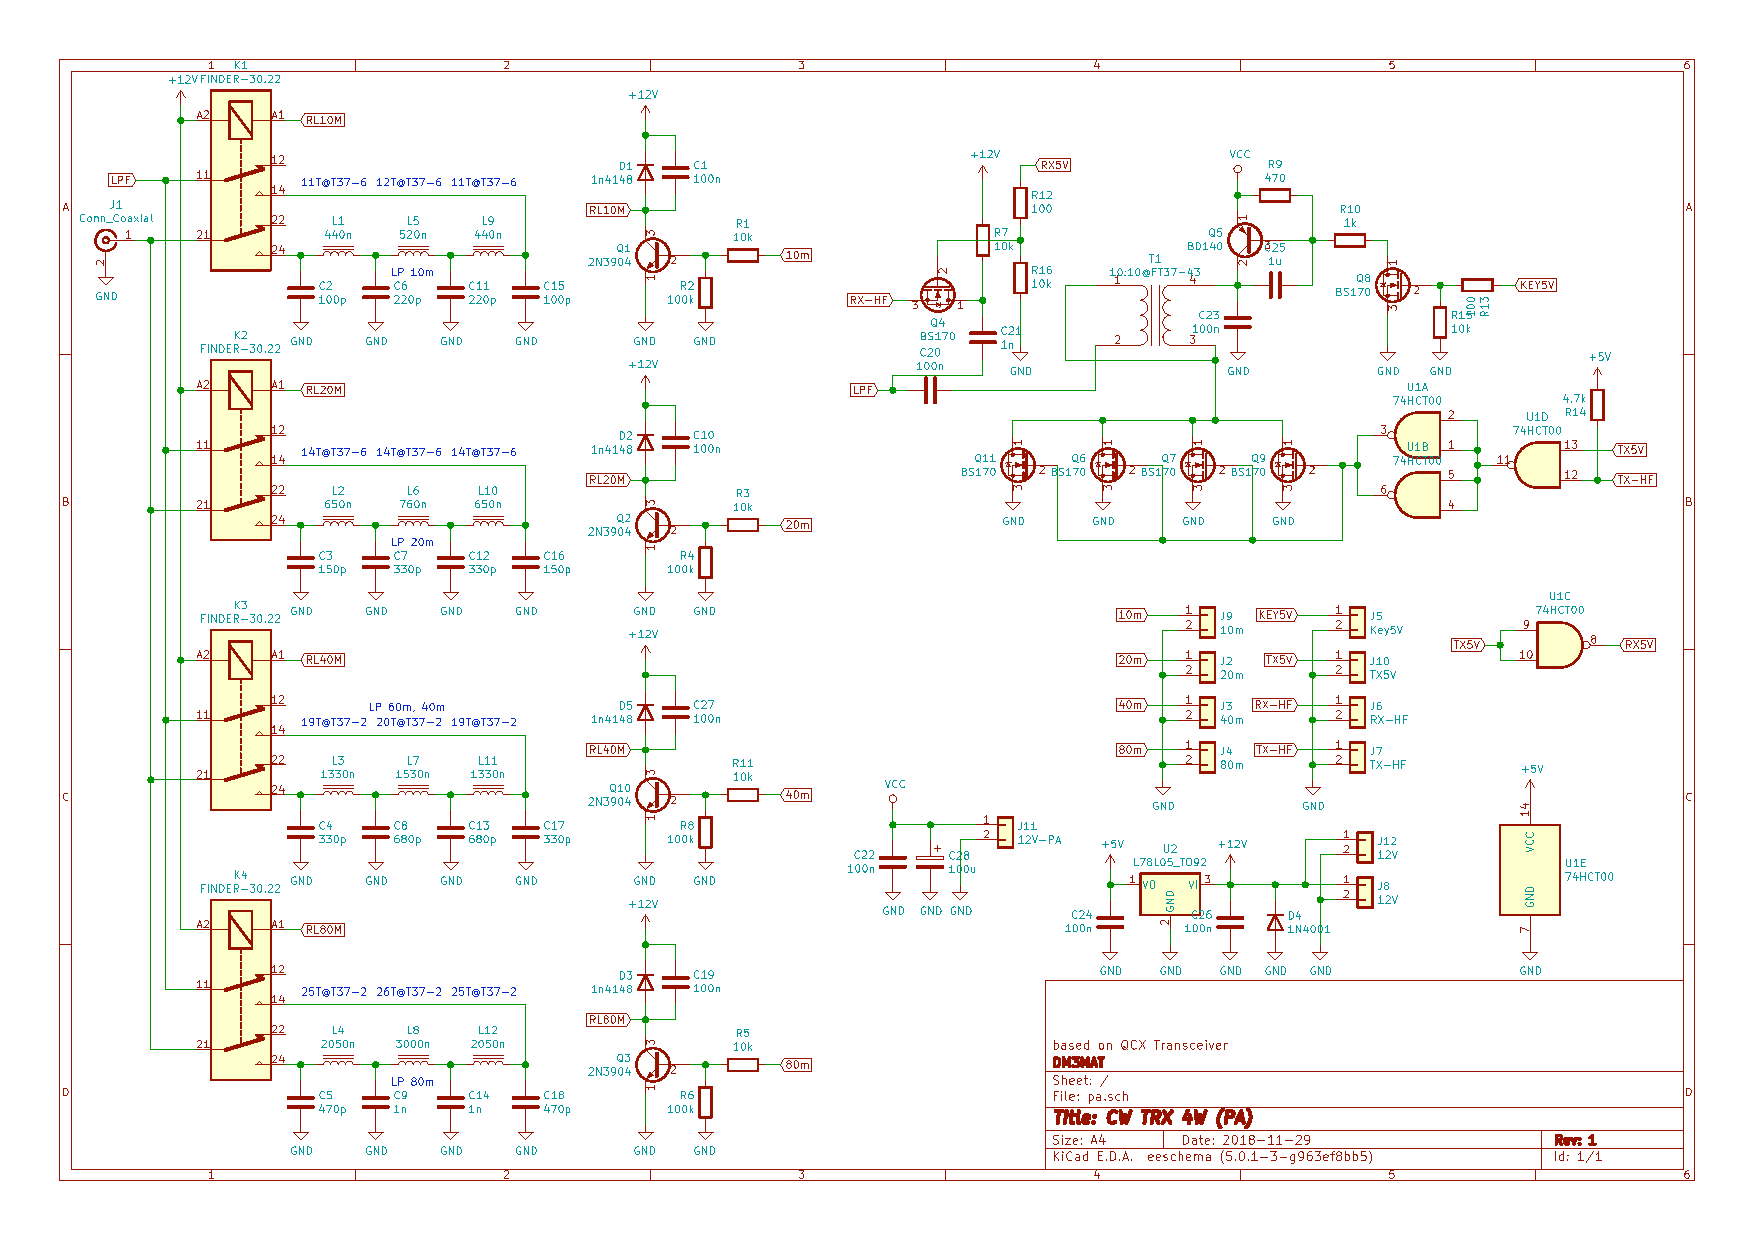
\includepdf[landscape=true]{fig/pa_scm.pdf}
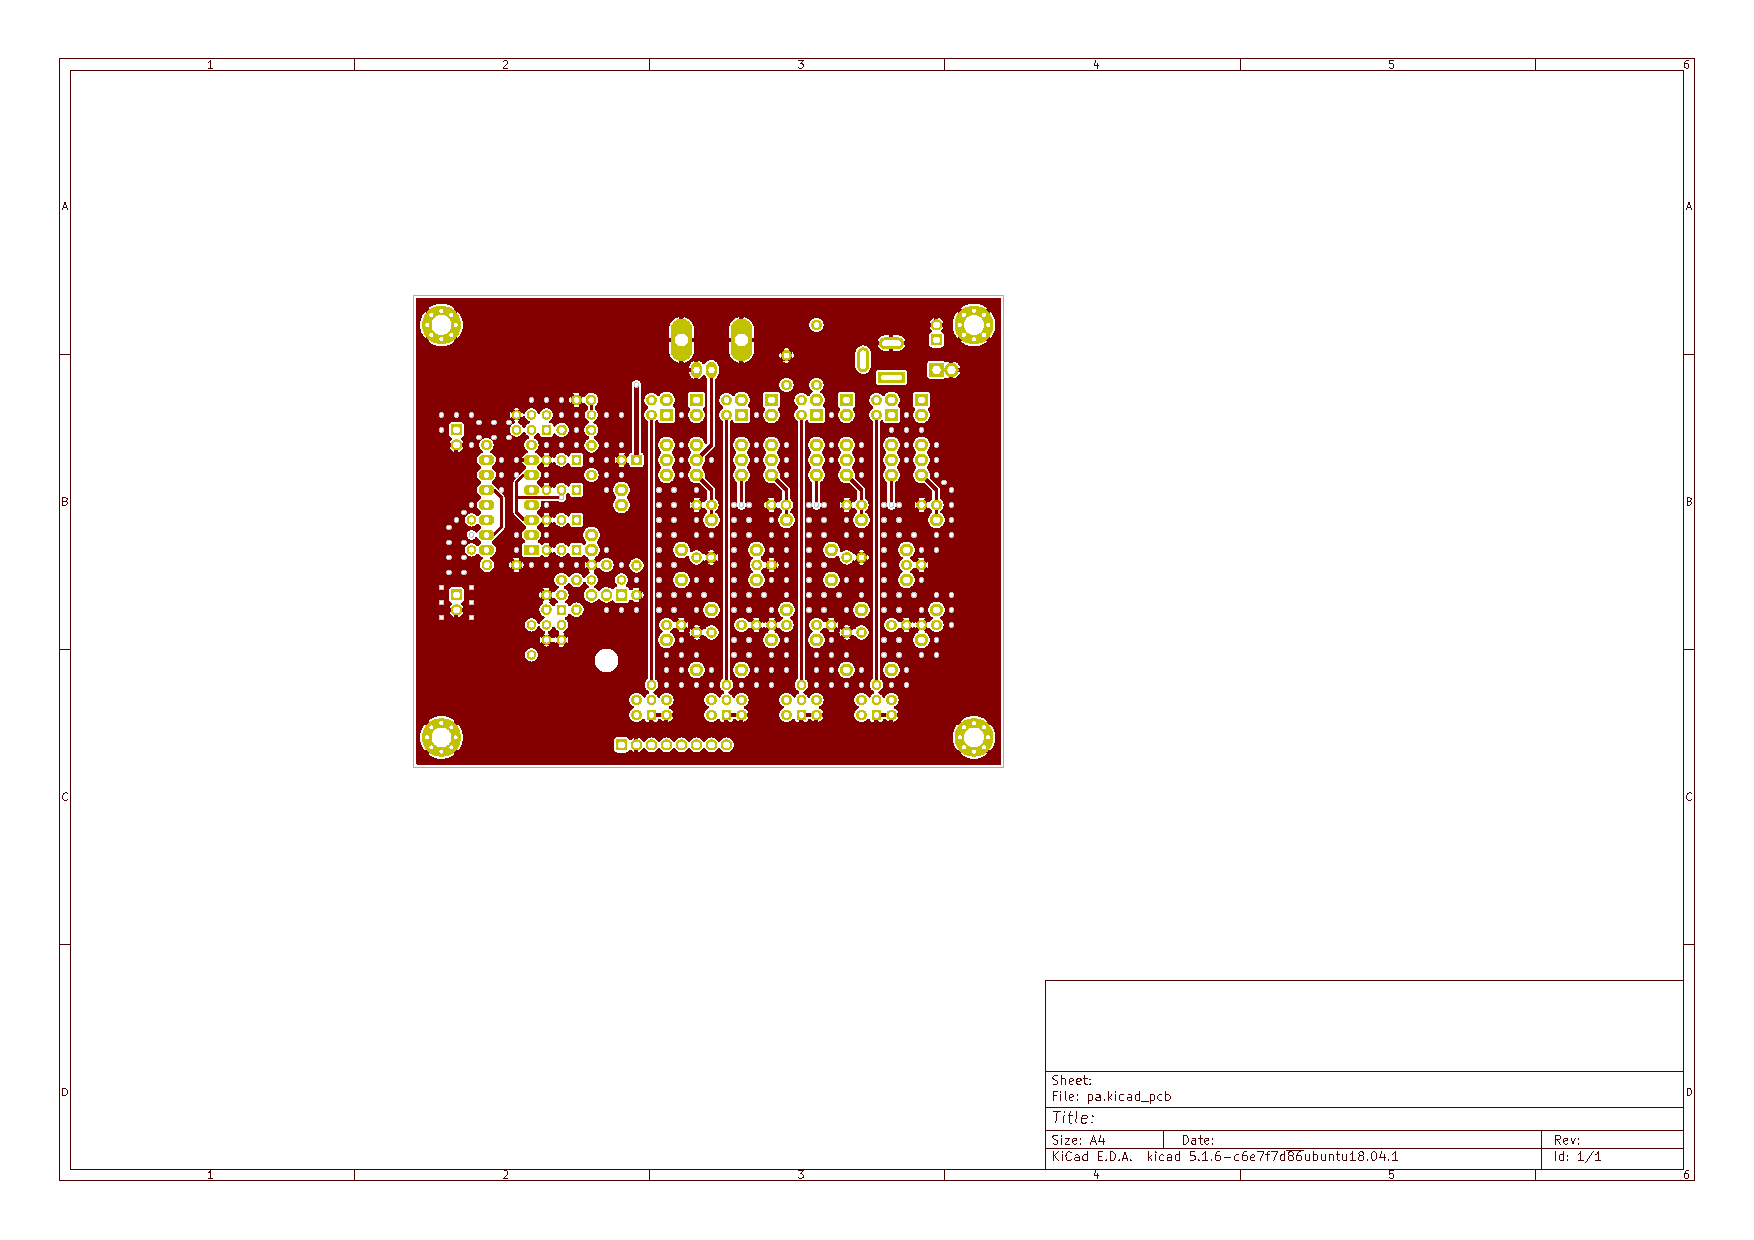
\includepdf[pages={1,2,3},landscape=true]{fig/pa_brd.pdf}
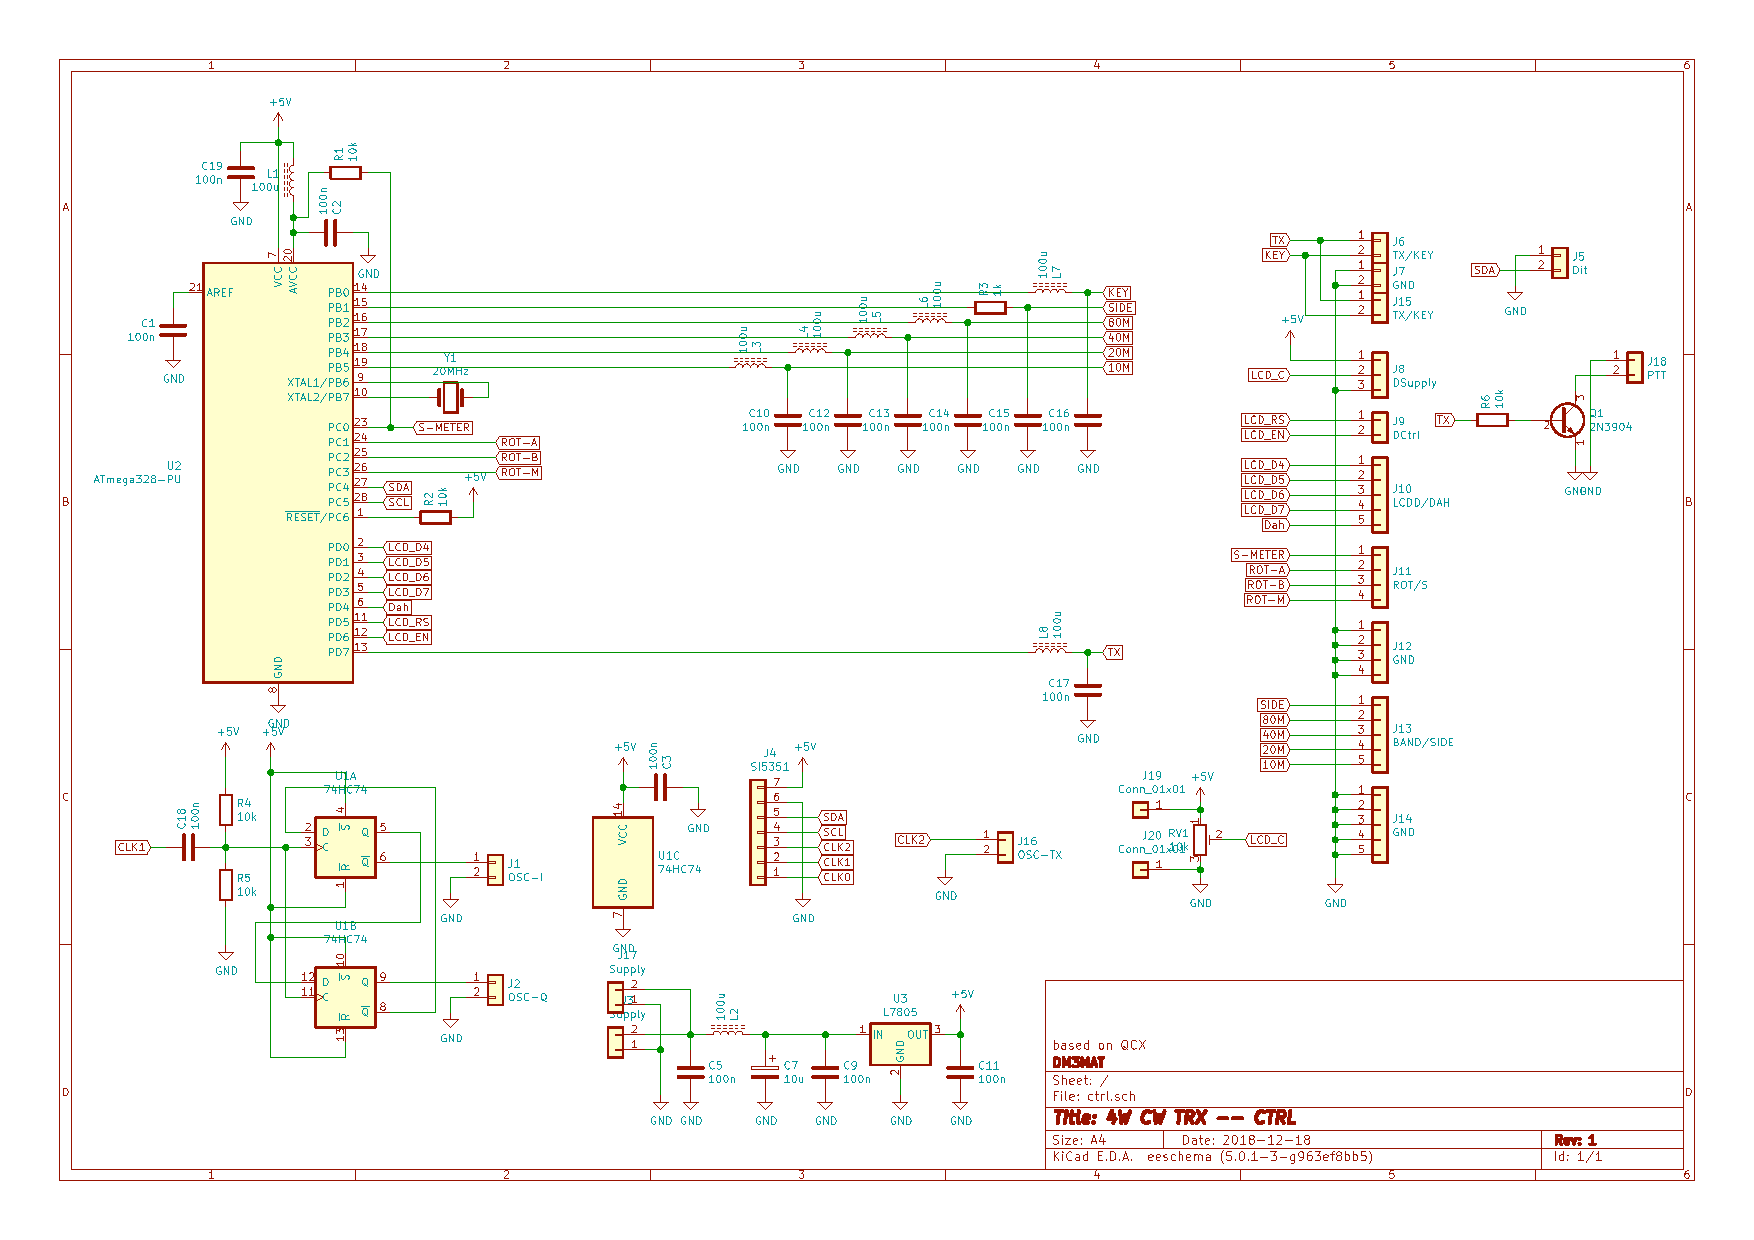
\includepdf[landscape=true]{fig/crtl_scm.pdf}
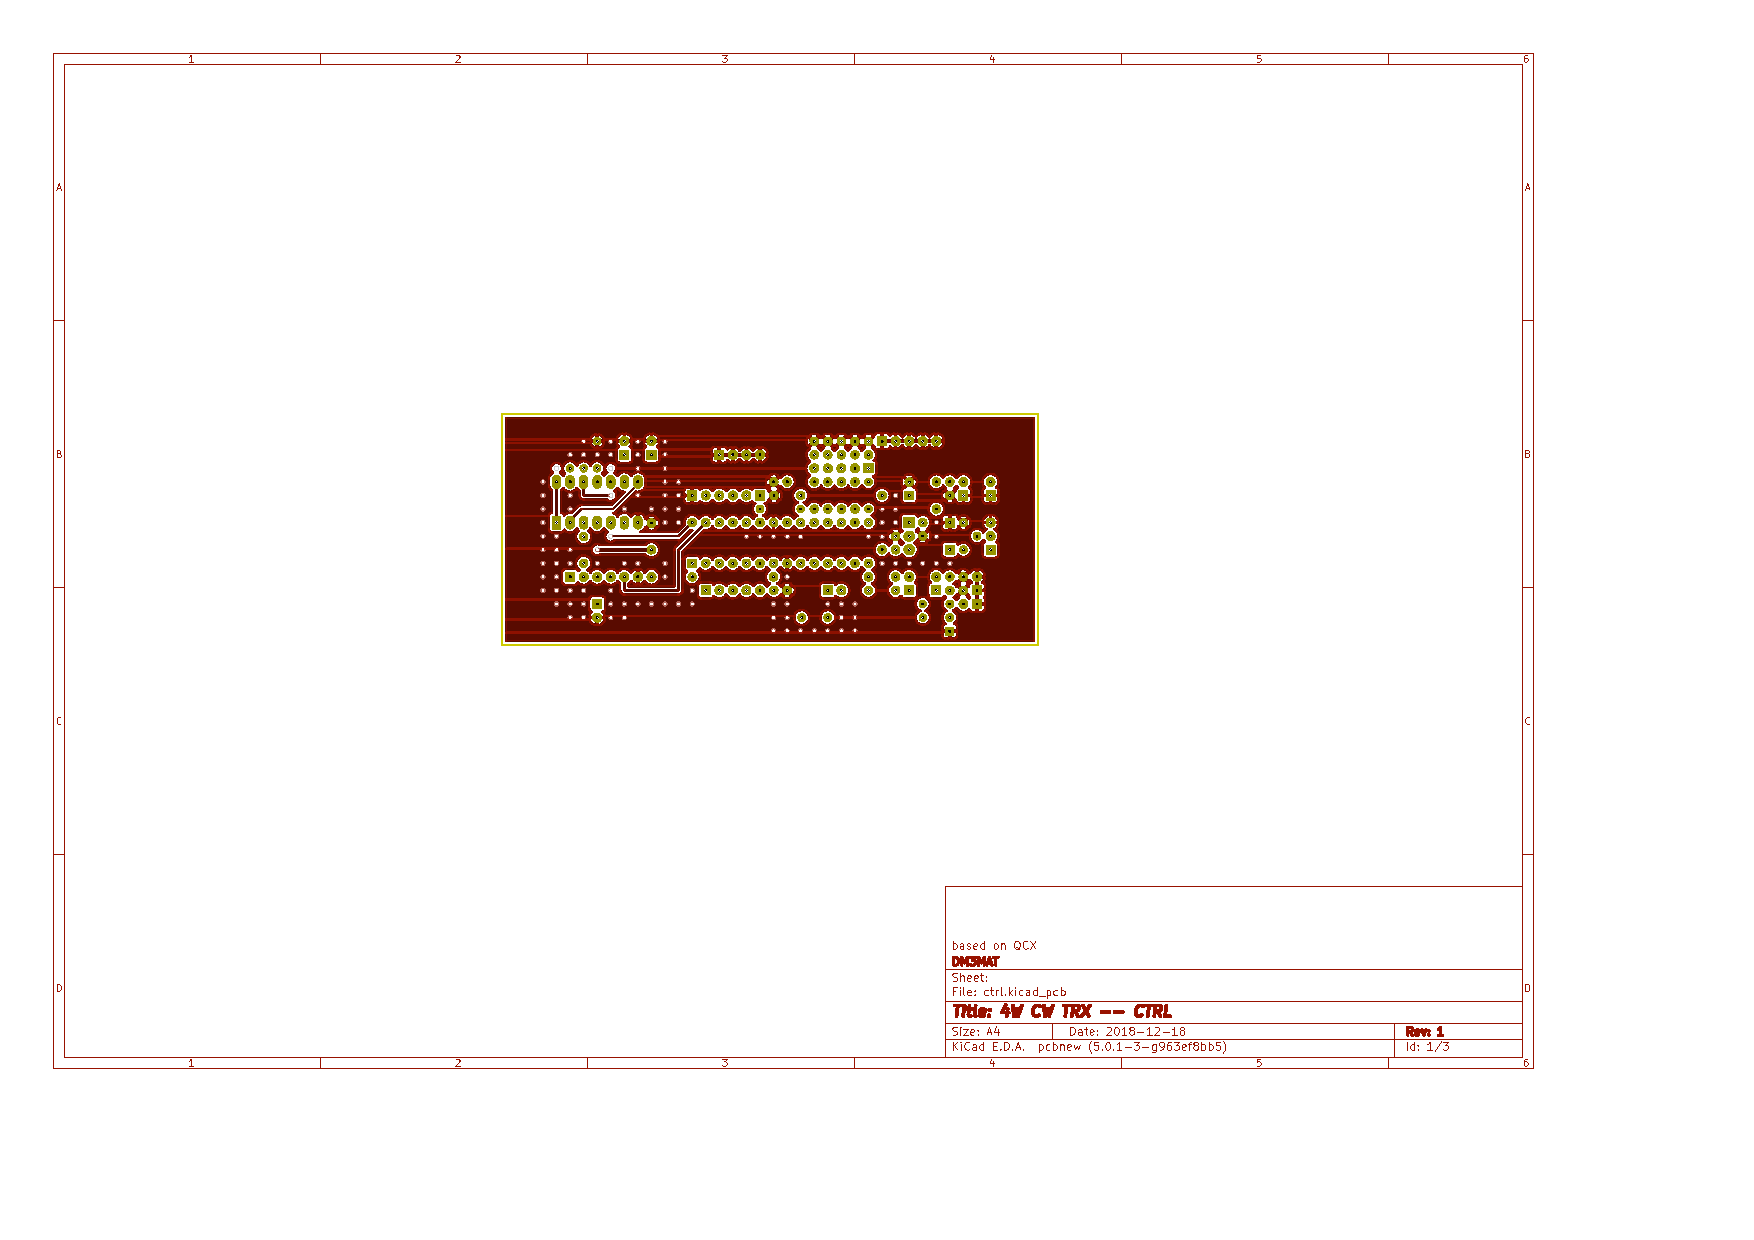
\includepdf[pages={1,2,3},landscape=true]{fig/ctrl_brd.pdf}
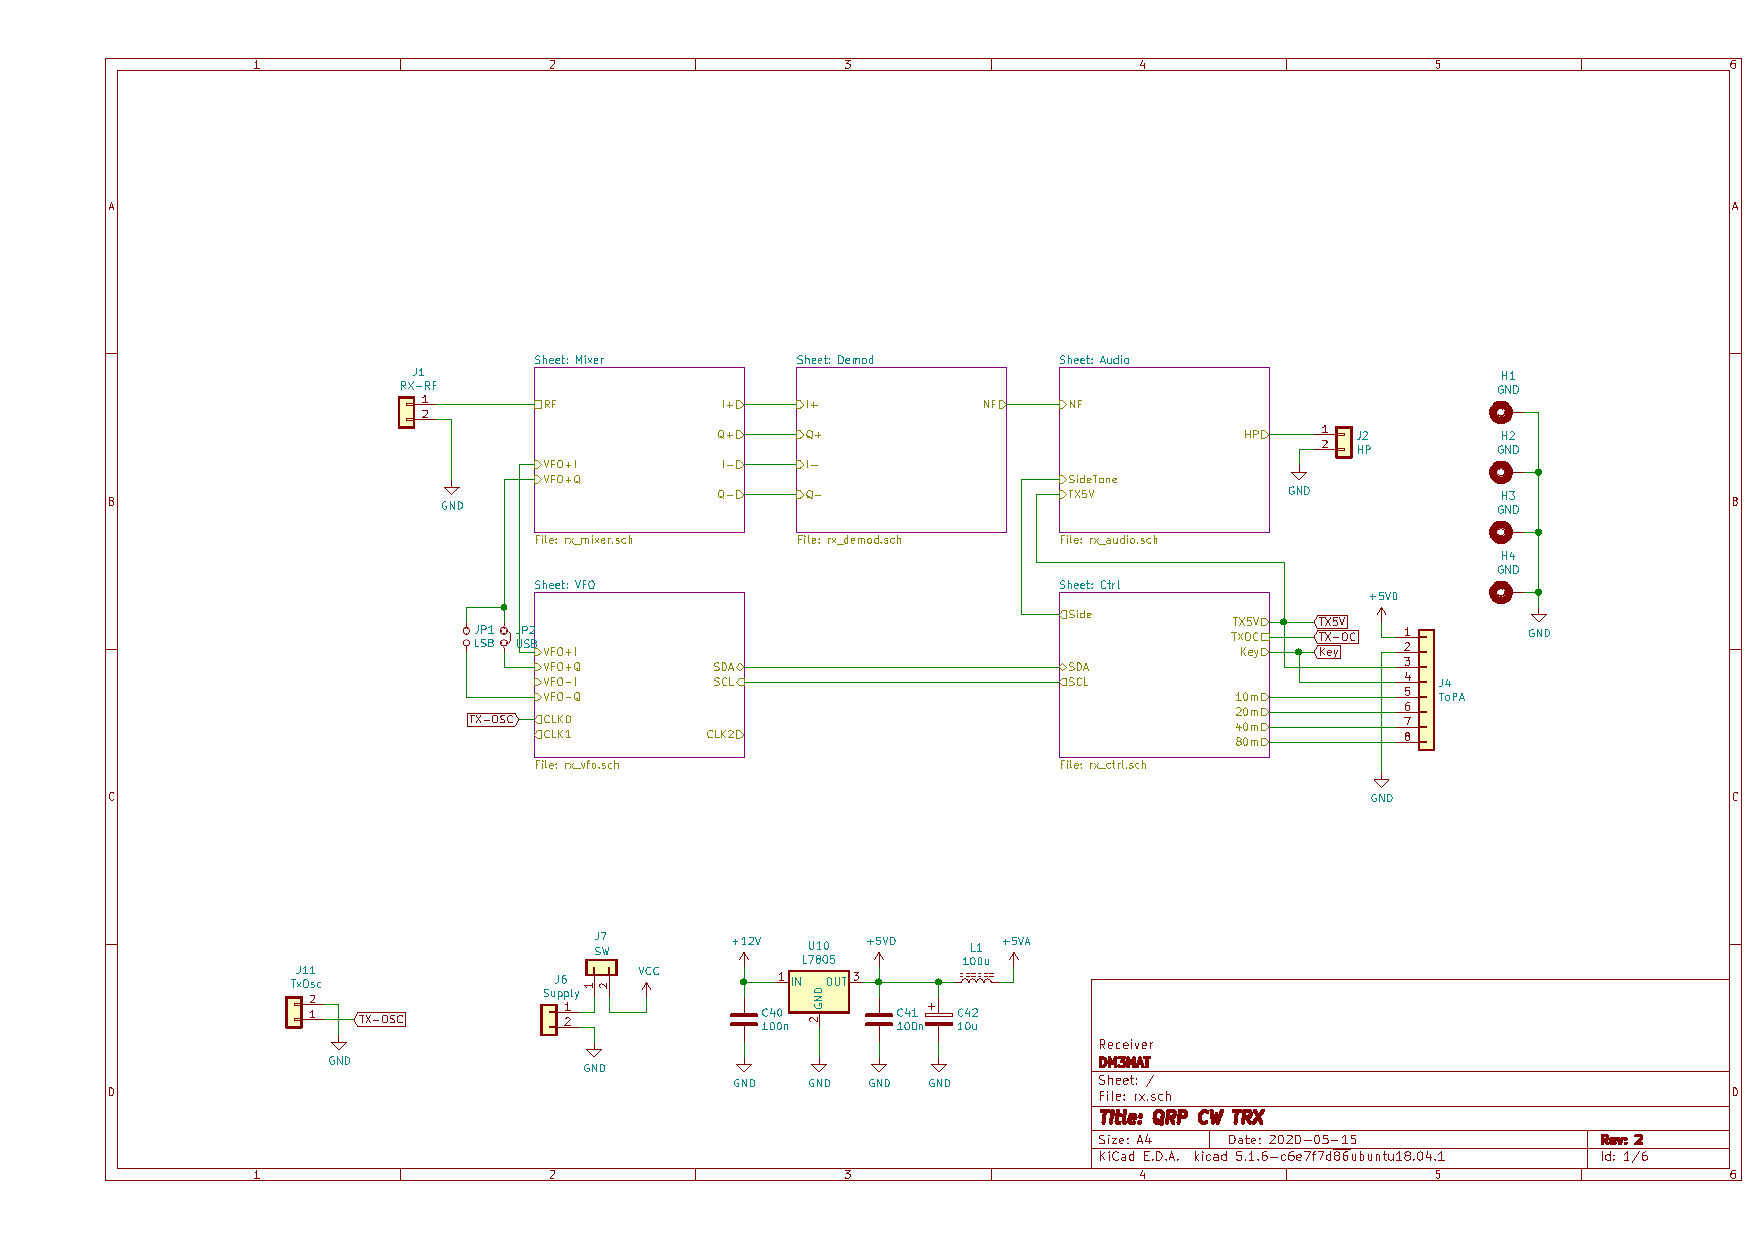
\includepdf[landscape=true]{fig/rx_scm.pdf}
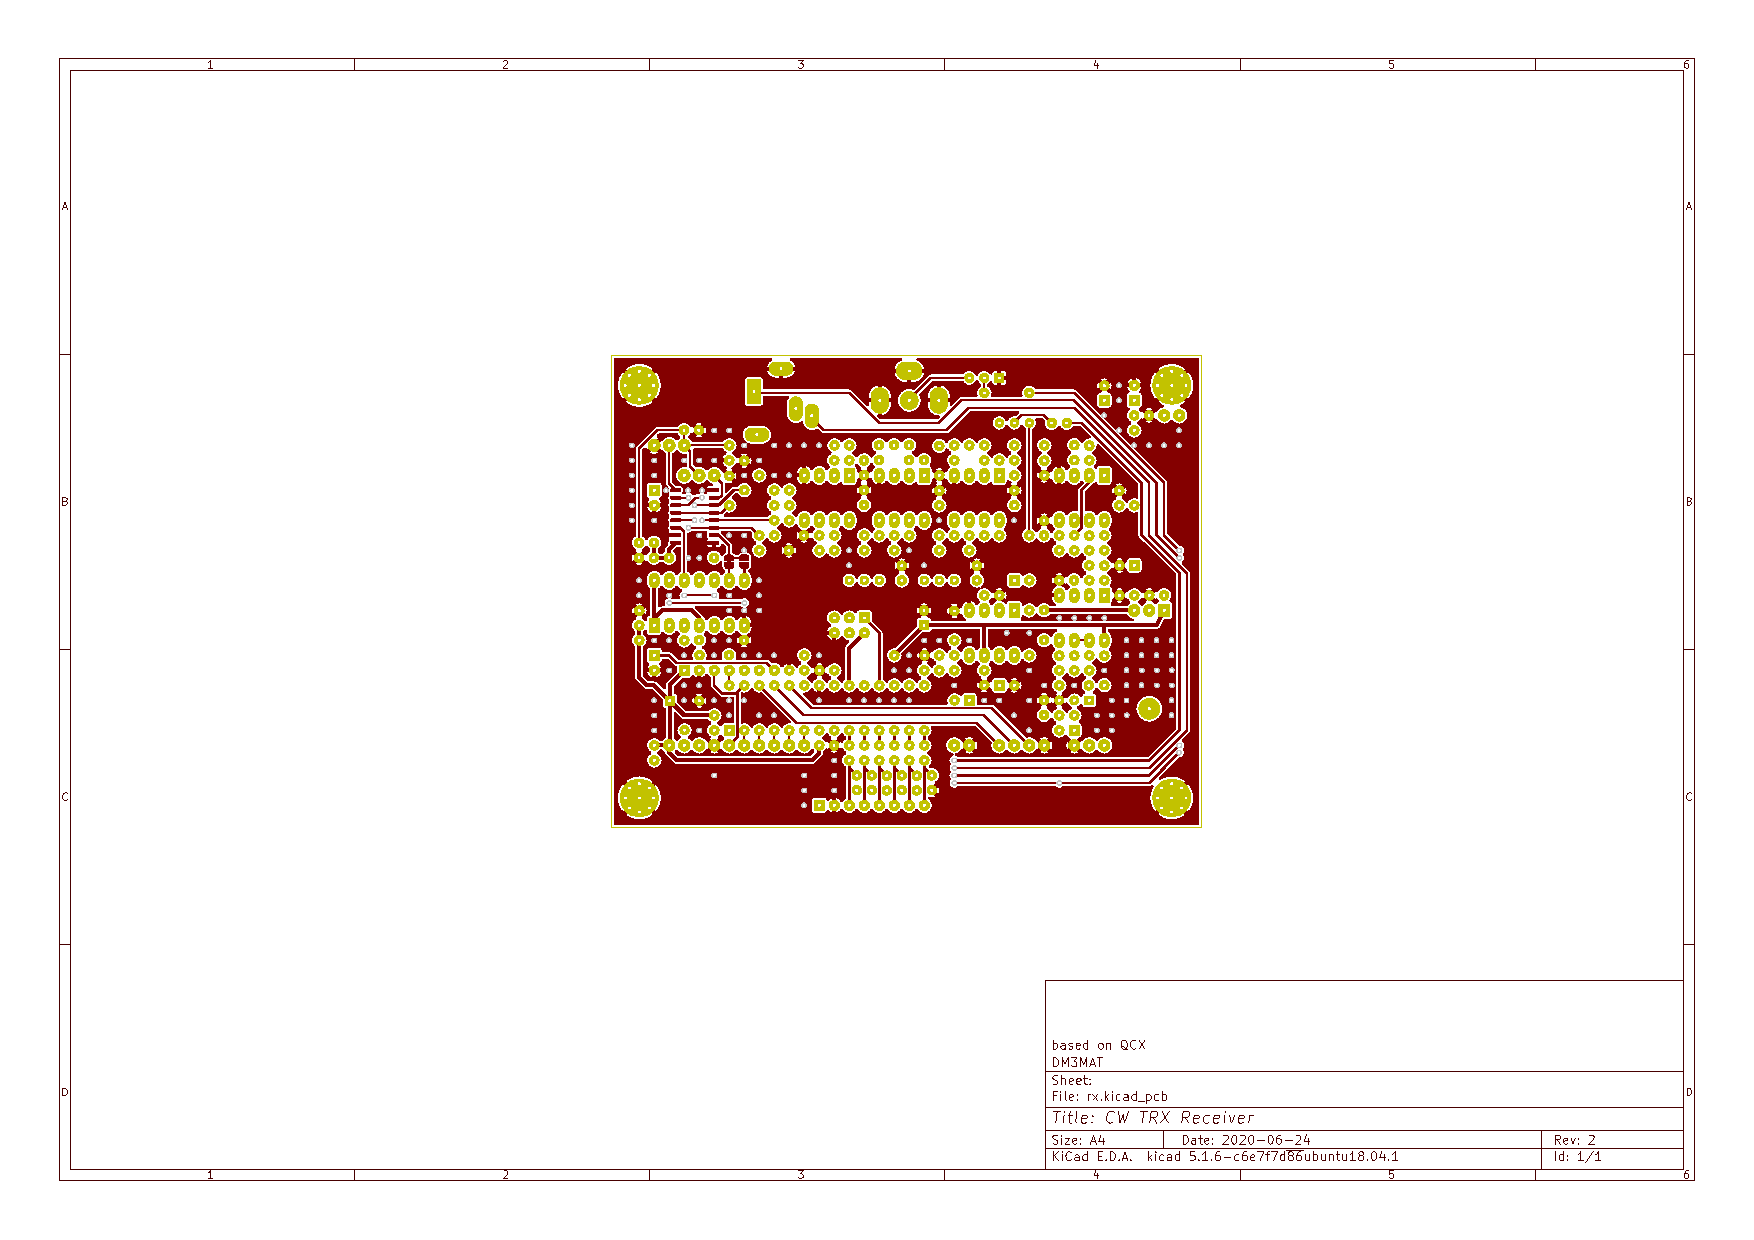
\includepdf[pages={1,2,3},landscape=true]{fig/rx_brd.pdf}
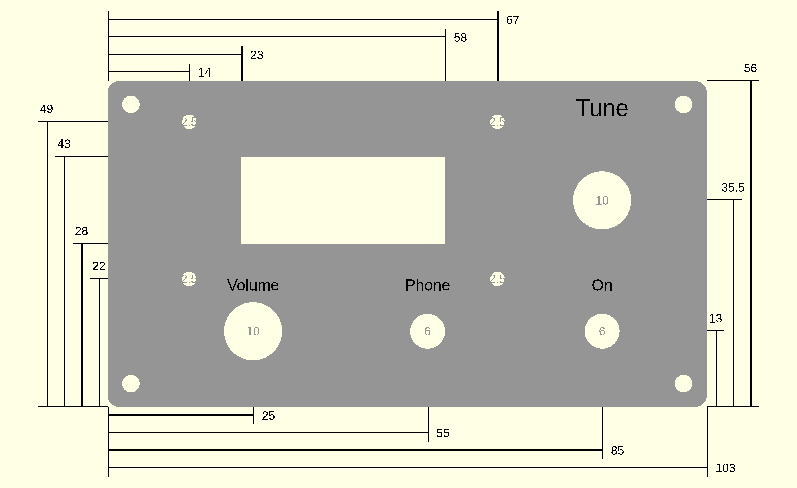
\includepdf[landscape=true]{fig/FrontPanel.png}
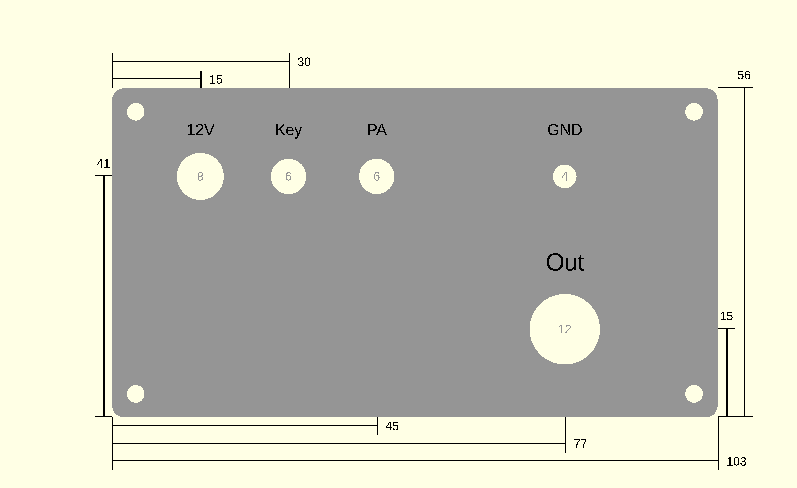
\includepdf[landscape=true]{fig/BackPanel.png}
\end{document}